\documentclass[11pt]{article}

\usepackage[margin=1in]{geometry}
\usepackage{amsmath}
\usepackage{amssymb}
\usepackage{booktabs}
\usepackage{graphicx}
\usepackage{microtype}
\usepackage{xurl}
\usepackage[hidelinks]{hyperref}
\setlength{\emergencystretch}{3em}

\title{Model comparison: the NIMBY benchmark and the fertility extension}
\date{March 20, 2026}

\begin{document}
\maketitle

\section{The model}

This note takes the model section of Gross and Chivers (2025) as the baseline object and isolates
the changes required to introduce fertility. The baseline NIMBY model is a life-cycle model with
housing and debt choice. Households differ by age, liquid wealth, housing, and idiosyncratic
income, and political support for additional housing supply is determined by the effect of a
small, persistent change in house prices on expected lifetime utility.

The fertility extension preserves that structure. Real estate firms, the neighborhood voting
problem, and the median-voter equilibrium condition remain in place. What changes is the
household problem. The household state is augmented with family states, and the flow utility from
housing is modified so that children at home reduce effective housing services through crowding.

\subsection{Household's problem}

Consider a household of age $j$ with liquid assets $b_t$, housing $a_t$, and income state $z_t$.
In the NIMBY benchmark, lifetime utility is
\begin{equation}
\sum_{j=0}^{J}\beta^{j}u(c_j, H_j) + \beta^{J+1}v(w_{J+1}),
\end{equation}
where $H_t$ denotes housing services from owner-occupied or rented housing and terminal utility is
the same warm-glow bequest motive used in the baseline paper.

For the benchmark comparison considered here, the NIMBY flow utility is
\begin{equation}
u^{N}_t = \log c_t + s_h \log H_t - \text{penalty}_t,
\end{equation}
with the terminal branch adding the bequest term
\begin{equation}
v(w_{t+1}) = \psi \log w_{t+1}.
\end{equation}

The fertility extension adds two family states:
\begin{itemize}
\item $p_t \in \{0,1,2,3+\}$, parity, or children ever born.
\item $h_t \in \{0,1,2,3\}$, children currently at home.
\end{itemize}

The state vector therefore changes from
\begin{equation}
\mathbf{s}^{N}_t = \{b_t, a_{t-1}, z_t\}
\end{equation}
to
\begin{equation}
\mathbf{s}^{F}_t = \{b_t, a_{t-1}, z_t, h_t, p_t\}.
\end{equation}

The key change is that housing enters utility through effective housing services rather than raw
housing services. Let
\begin{equation}
H_t^{eff} = \frac{H_t}{(1+\lambda_c h_t)^{\psi_c}}.
\end{equation}
Then, absent a birth in the current period, the fertility-extension flow utility is
\begin{equation}
u^{F,0}_t = \log c_t + s_h \log H_t^{eff} + \nu_h h_t - \text{penalty}_t.
\end{equation}

If a birth occurs in the current period, the newborn counts immediately in both the crowding term
and the child-utility term:
\begin{equation}
u^{F,1}_t = \log c_t + s_h \log \left(\frac{H_t}{(1+\lambda_c(h_t+1))^{\psi_c}}\right)
+ \nu_h(h_t+1) + \phi(p_t) - \kappa_0 - \kappa_q q_t - \text{penalty}_t.
\end{equation}
Here $\phi(p_t)$ is parity-specific birth utility, $\kappa_0$ is the direct birth cost, and
$\kappa_q q_t$ is the housing-price-sensitive birth cost.

Births therefore arise from a comparison between the birth and no-birth branches of the
household problem.

The family-state transitions are
\begin{equation}
p_{t+1} = \min\{p_t + \mathbf{1}\{\text{birth}\}, 3+\},
\end{equation}
\begin{equation}
h_{t+1} = h_t + \mathbf{1}\{\text{birth}\} - \ell_t,
\end{equation}
where $\ell_t \in \{0,1\}$ is a reduced-form leave-home shock. This separation between parity and
children-at-home is the key modeling distinction in the corrected benchmark. A household's
completed fertility is permanent, while the crowding state that governs housing demand is
temporary.

The baseline NIMBY model is nested exactly when the fertility block is shut off. The precise
parameter restrictions used for that nesting result are reported in the appendix.

\subsection{Real estate firms}

The real-estate block is unchanged. Rental housing is supplied competitively and the rental price
is pinned down by the user cost of housing and expected capital gains. The zero-profit condition
therefore remains
\begin{equation}
p_t^{rent} = \phi^{rent} + r_t^a p_t^h - \Delta p_{t+1}^h.
\end{equation}

\subsection{Housing supply}

The local political mechanism is also unchanged. Households vote over a small, persistent change
in local housing supply, taking the induced change in house prices as given. A household supports
lower housing supply if a small increase in the house price raises expected lifetime utility:
\begin{equation}
V_j(\mathbf{s}; p^h+\epsilon^p) - V_j(\mathbf{s}; p^h) + \sigma \geq 0.
\end{equation}

What changes is the object inside the vote calculation. In the fertility model the value
function depends on both the housing portfolio and the household's family state, so the same
price perturbation is filtered through an enlarged state space and a different utility function.

\subsection{The median voter theorem}

Applying the same median-voter logic as in the NIMBY benchmark, the equilibrium house price
satisfies
\begin{equation}
\int g(\mathbf{s}; p_t^h)\Theta(\mathbf{s}; p^h)\, d\mathbf{s} = 0.5,
\end{equation}
where
\begin{equation}
\Theta(\mathbf{s}; p^h) =
\mathbf{1}_{\{V_j(\mathbf{s}; p^h+\epsilon^p)-V_j(\mathbf{s}; p^h)+\sigma \geq 0\}}.
\end{equation}

The median-voter condition is therefore unchanged in form. The fertility extension matters because
it shifts both the support function $\Theta(\cdot)$ and the stationary state distribution
$g(\cdot)$.

\subsection{Equilibrium}

The political-economic equilibrium consists of household value functions, tenure and portfolio
policies, births, the stationary distribution of households over the augmented state vector, and
the house price that makes the median voter indifferent to a small change in supply. Relative to
the baseline NIMBY benchmark, the fertility extension adds family-state policies and family-state
distributions, but leaves the equilibrium concept itself unchanged.

\section{Benchmark comparison}

\subsection{Exact nesting result}

The first benchmark fact is exact nesting. When the fertility block is shut off, the fertility
model reproduces the upstream NIMBY steady state exactly. The implementation details behind that
verification are reported in the appendix.

\begin{table}[htbp]
\centering
\begin{tabular}{lc}
\toprule
Check & Gap \\
\midrule
Distance gap & 0 \\
Vote gap & 0 \\
Debt gap & 0 \\
\bottomrule
\end{tabular}
\caption{Reproduction check: the fertility solver nests the NIMBY benchmark exactly in the shutoff case.}
\end{table}

\subsection{What changes in the benchmark}

Using the common $rbPos=0.03$ convention and tracing political support over the same house-price
grid, the equilibrium crossing shifts materially once fertility is active.

\begin{table}[htbp]
\centering
\begin{tabular}{lcc}
\toprule
Object & NIMBY benchmark & Fertility benchmark \\
\midrule
Crossing house price & 2.326287 & 1.751853 \\
Vote at refined price & 0.002227 & 0.008446 \\
Vote per unit mass at refined price & 0.000349 & 0.001370 \\
Stationary household mass & 6.387684 & 6.163346 \\
Debt stock at refined price & -4.177670 & 44.406591 \\
Rent share at refined price & 3.963530 & 2.866941 \\
Average birth rate & -- & 0.597710 \\
\bottomrule
\end{tabular}
\caption{Steady-state benchmark comparison at the refined crossing implied by each model.}
\end{table}

The central quantitative result is that the fertility extension shifts the support schedule toward
lower house prices. The equilibrium crossing moves from 2.326287 in the NIMBY benchmark to
1.751853 in the fertility benchmark. The interpretation is straightforward. In the baseline
NIMBY model households care about house prices through portfolio and tenure considerations. In the
fertility extension they also care about the effect of house prices on crowding and the cost of
family formation. That additional margin makes high house prices less politically acceptable.

\begin{figure}[htbp]
\centering
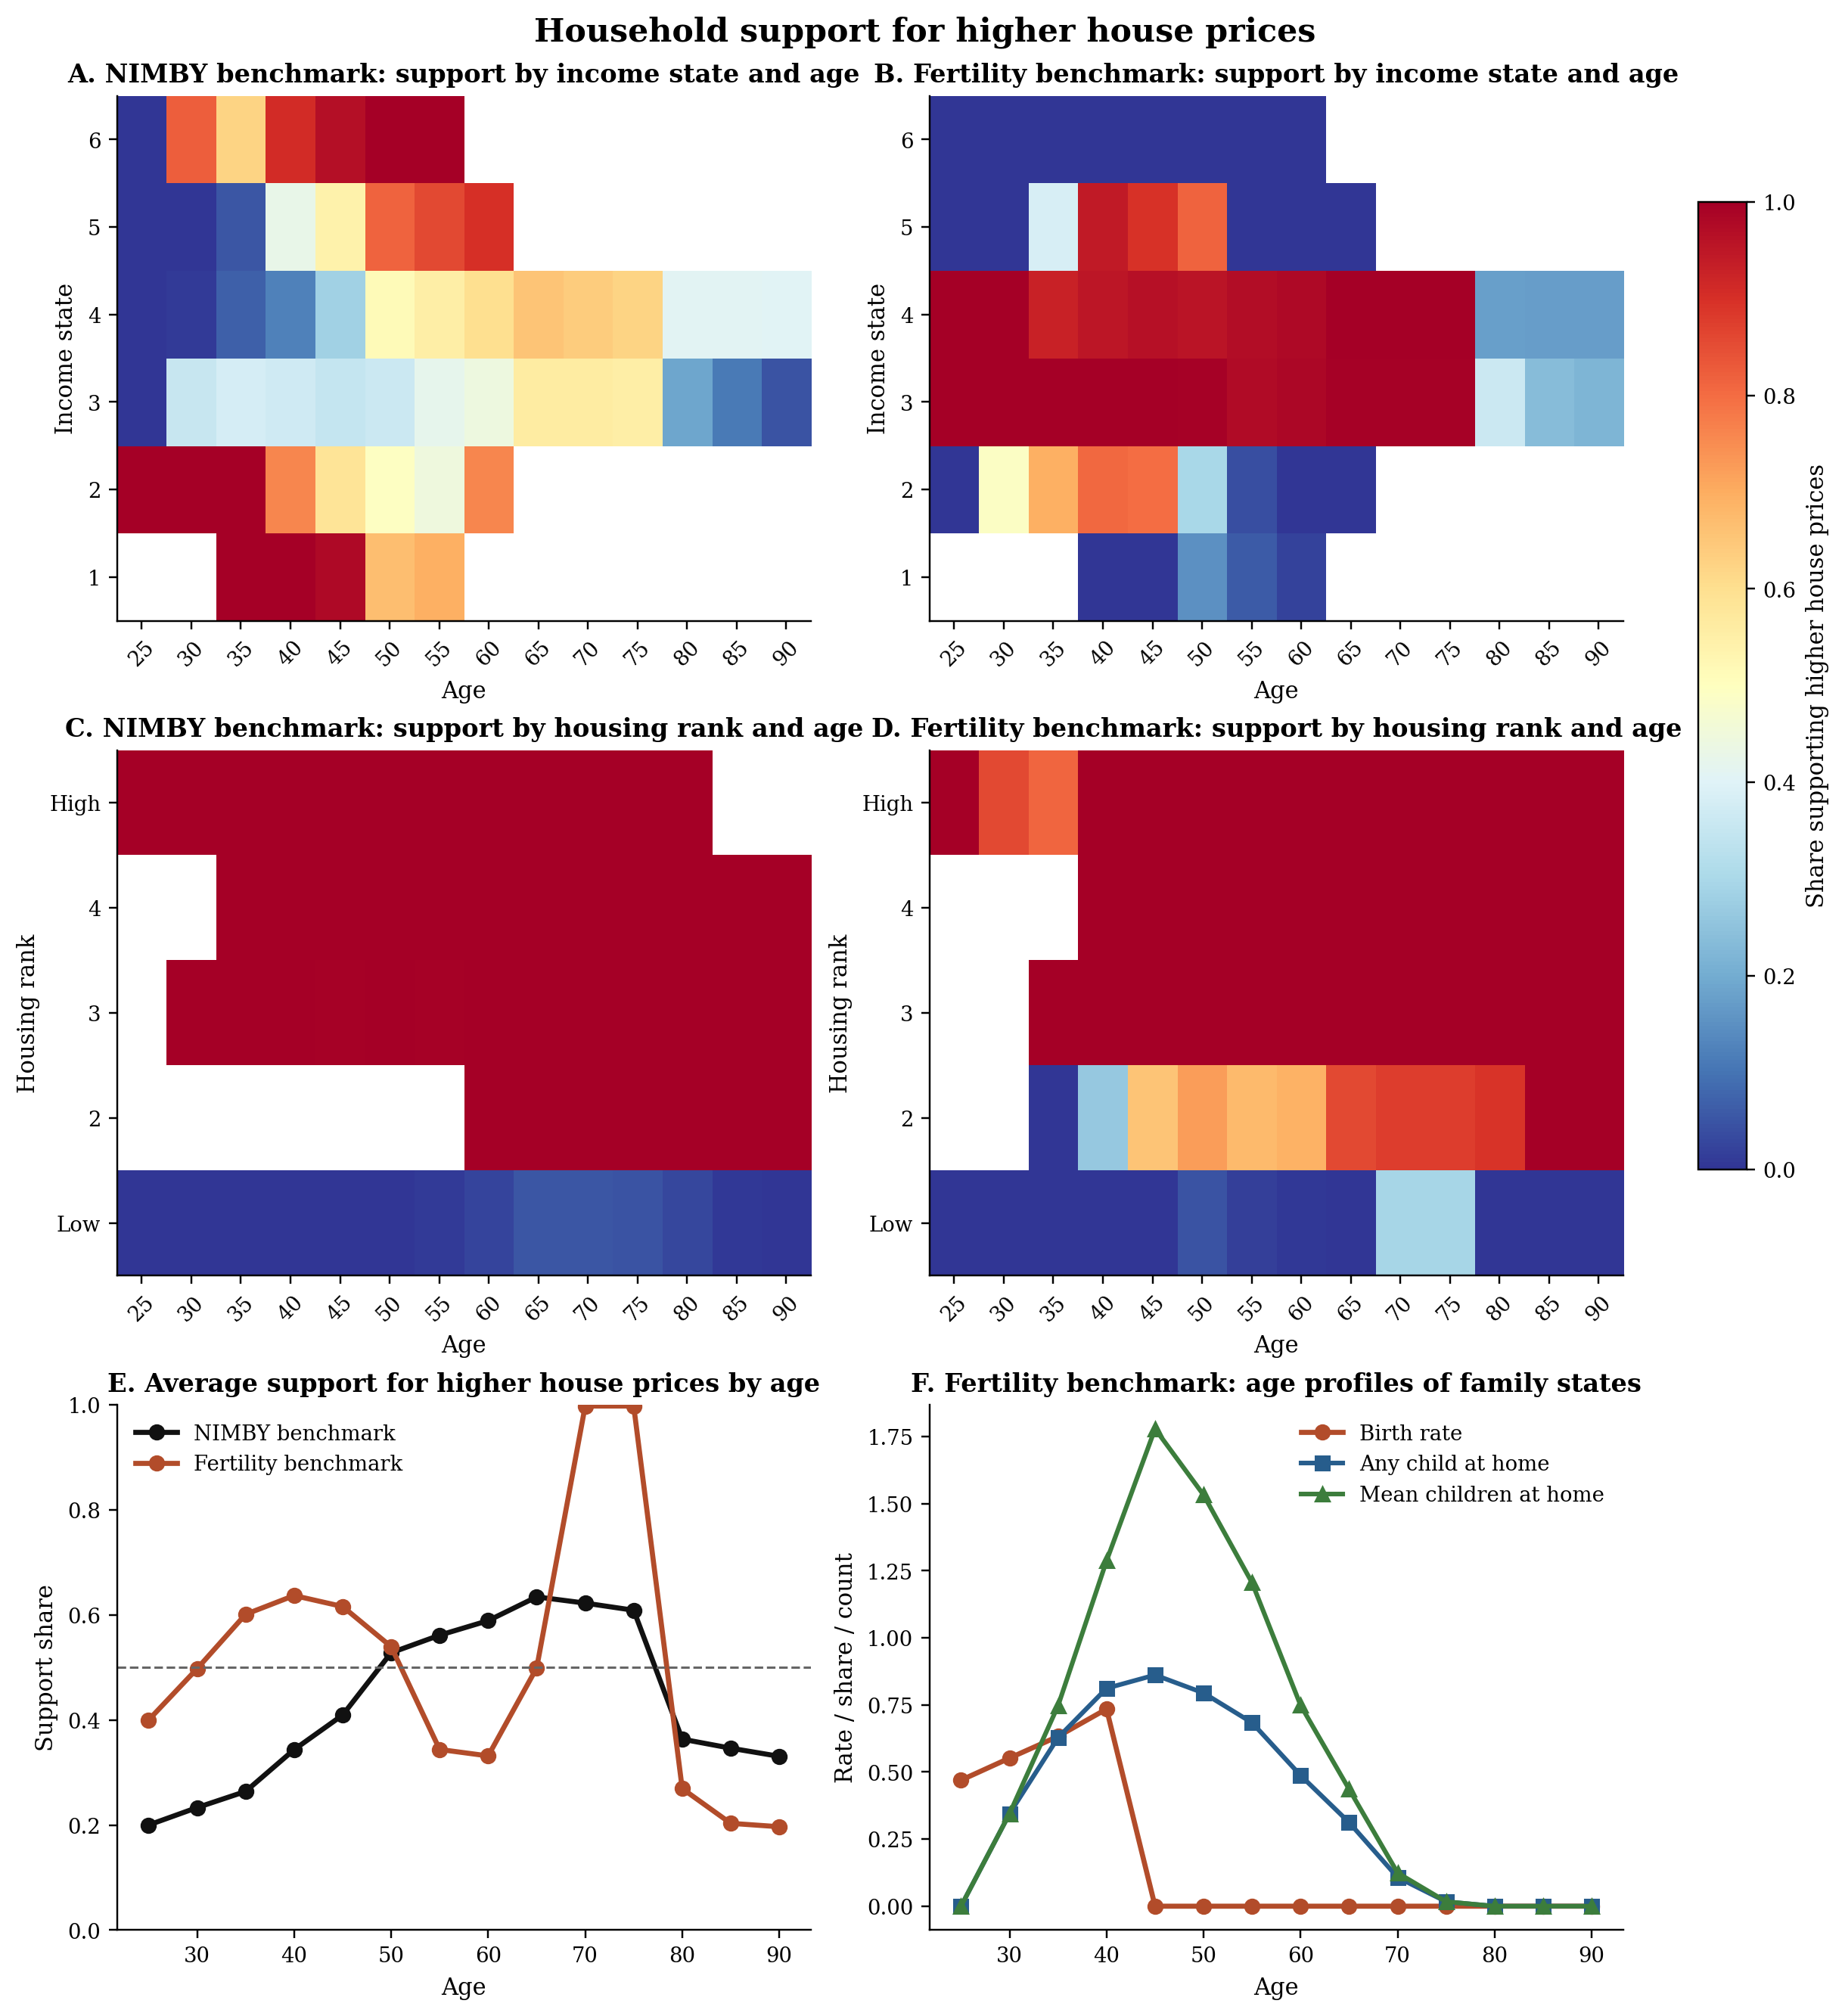
\includegraphics[width=\textwidth]{nimby_vs_fertility_household_support.png}
\caption{Household support for higher house prices. Panels A--D redraw the NIMBY paper's voting
figures using the baseline NIMBY steady state and the fertility steady state. Panel E shows the
age profile of support in the two benchmarks. Panel F adds the family-state profiles that are
unique to the fertility extension.}
\end{figure}

\begin{figure}[htbp]
\centering
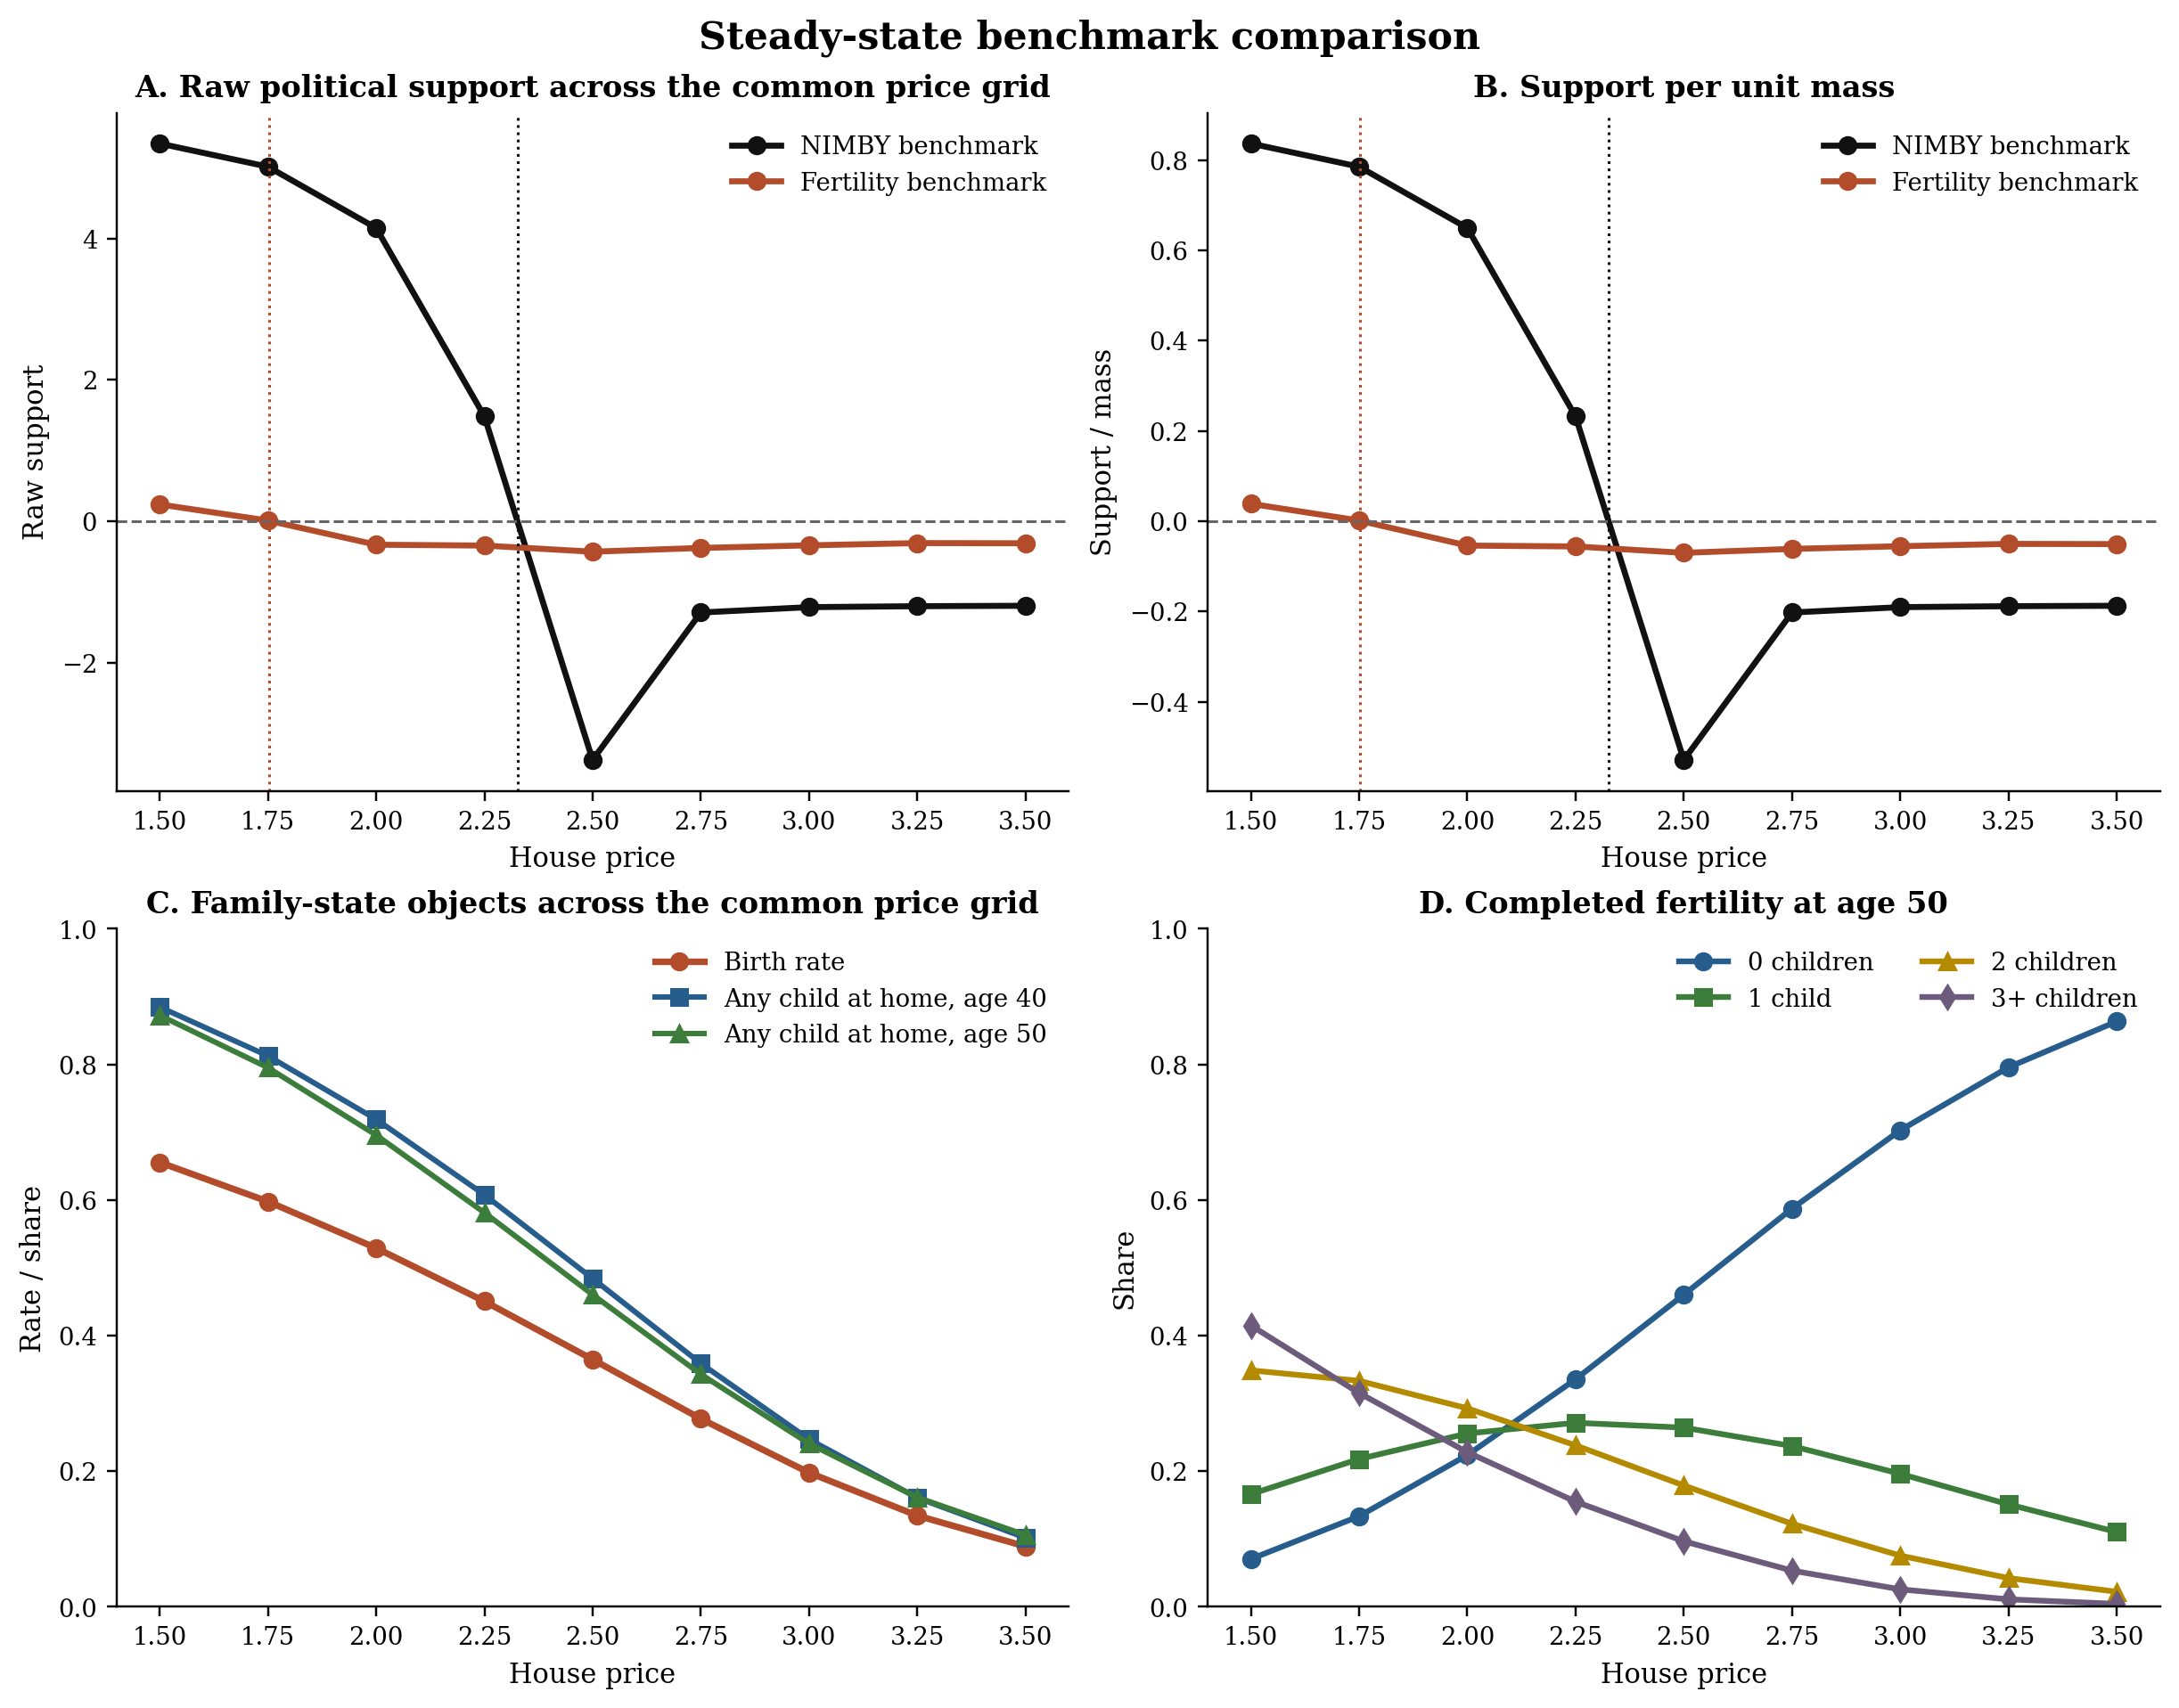
\includegraphics[width=\textwidth]{nimby_vs_fertility_benchmark_objects.png}
\caption{Steady-state benchmark comparison on the common house-price grid. The top row traces the
raw vote schedule and the vote-per-mass schedule in the two models. The bottom row shows the
family-state objects that move with house prices in the fertility benchmark.}
\end{figure}

\section{Temporary birthrate increase}

To connect the steady-state comparison to the original NIMBY paper's dynamic experiment, I impose
the same temporary baby-boom shock used in the upstream transition exercise: a 10 percent
increase in births for 10 periods. Figure 3 reports the resulting transition comparison. Panel A
shows the common imposed shock. Panels B and C compare the demographic and house-price responses
in the two models. Panels D and E add tenure-access responses, while Panel F isolates the
additional family-state responses that only exist in the fertility extension.

The central transition result is that the fertility extension produces a larger medium-run house
price response than the original NIMBY model under the same baby-boom shock. After normalizing
each model's house-price path by its own initial level, the average post-window price deviation is
about 2.0 percent in the NIMBY transition and about 5.1 percent in the fertility transition. At
the same time, the fertility model displays an additional family adjustment that the NIMBY model
does not contain: fertility rises during the boom by about 0.022 relative to baseline, then falls
slightly below baseline in later periods, while the stock of children at home remains temporarily
elevated.

The natural interpretation is that the baby boom does more than shift the age distribution. In the
fertility model it also changes current family crowding and the demand for housing space. That
extra family-demand channel amplifies the later tightening of the housing market relative to the
original NIMBY transition.

Because the current project-03 transition block still abstracts from an explicit tenure choice,
the homeownership panels in Figure 3 should be read as proxy objects. Each age bin is mapped into
a common age-profile of homeownership, and that schedule is then shifted by the model-implied
house-price path. Even with that conservative mapping, the fertility extension produces a much
larger deterioration in young homeownership access than the original NIMBY transition. The trough
in the young-homeownership response is about $-0.0107$ in the fertility transition, compared with
about $-0.0019$ in the NIMBY benchmark. The same ranking does not hold for older households. The
old-homeownership proxy in the fertility transition stays close to zero early on and reaches a
much smaller late decline than the NIMBY line.

\begin{figure}[htbp]
\centering
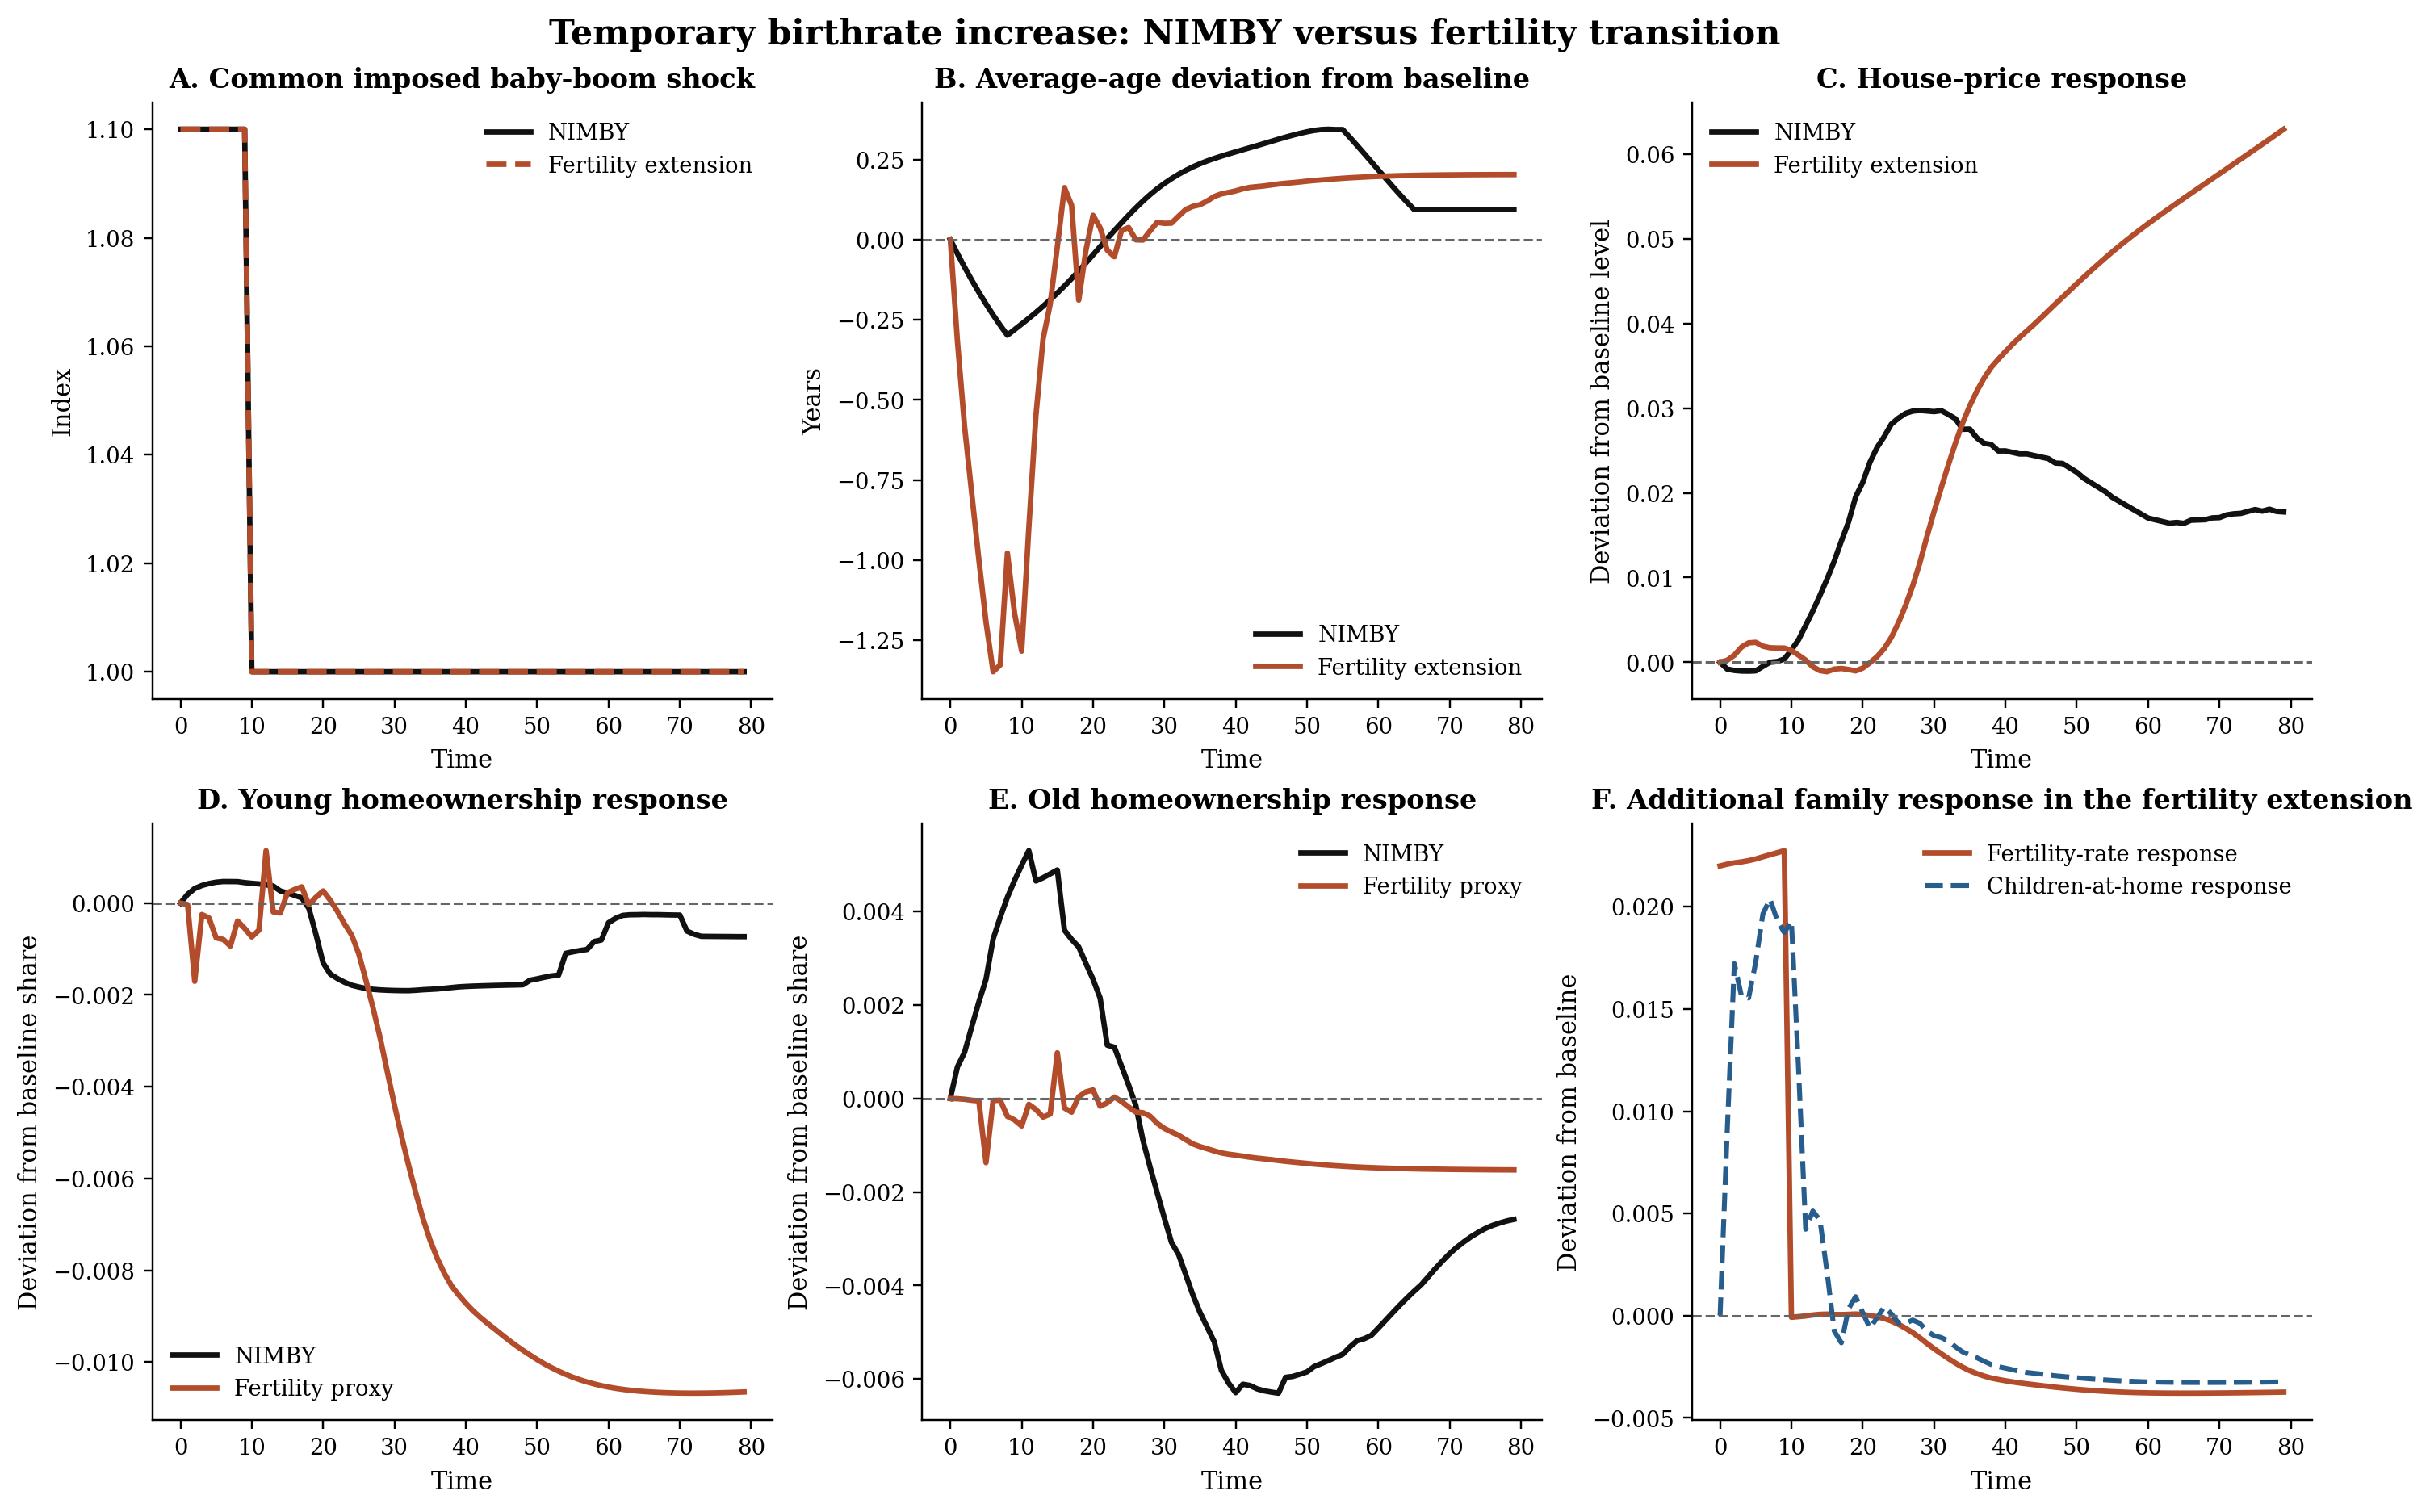
\includegraphics[width=\textwidth]{nimby_vs_fertility_baby_boom_transition.png}
\caption{Temporary birthrate increase: NIMBY versus fertility transition. Panel A shows the common
10 percent baby-boom shock for 10 periods. Panel B compares the average-age response. Panel C
compares the house-price response after normalizing each model by its initial house-price level.
Panels D and E compare young and old homeownership responses; the fertility lines are
composition-and-affordability tenure proxies because the current transition block does not solve
an explicit tenure choice. Panel F reports the additional family-state responses that only appear
in the fertility extension.}
\end{figure}

The original NIMBY paper also emphasizes cohort incidence. Figure 4 provides the closest current
counterpart on the fertility side. The NIMBY lines are the upstream cohort homeownership indices
for the boom generation, their parents, and their children. The fertility lines use the same
age-and-price tenure mapping described above, evaluated along those cohort age paths. They are
therefore access proxies, not structural cohort policy functions, but they are still informative
about incidence. The parent generation is barely affected. The boom generation loses some
homeownership access in midlife, and the child generation is hit most strongly, with the proxy
index falling to roughly $0.974$. That ordering matches the paper's intended mechanism: the
stronger house-price response in the fertility model is borne most heavily by later cohorts trying
to enter owner-occupation after the boom.

\begin{figure}[htbp]
\centering
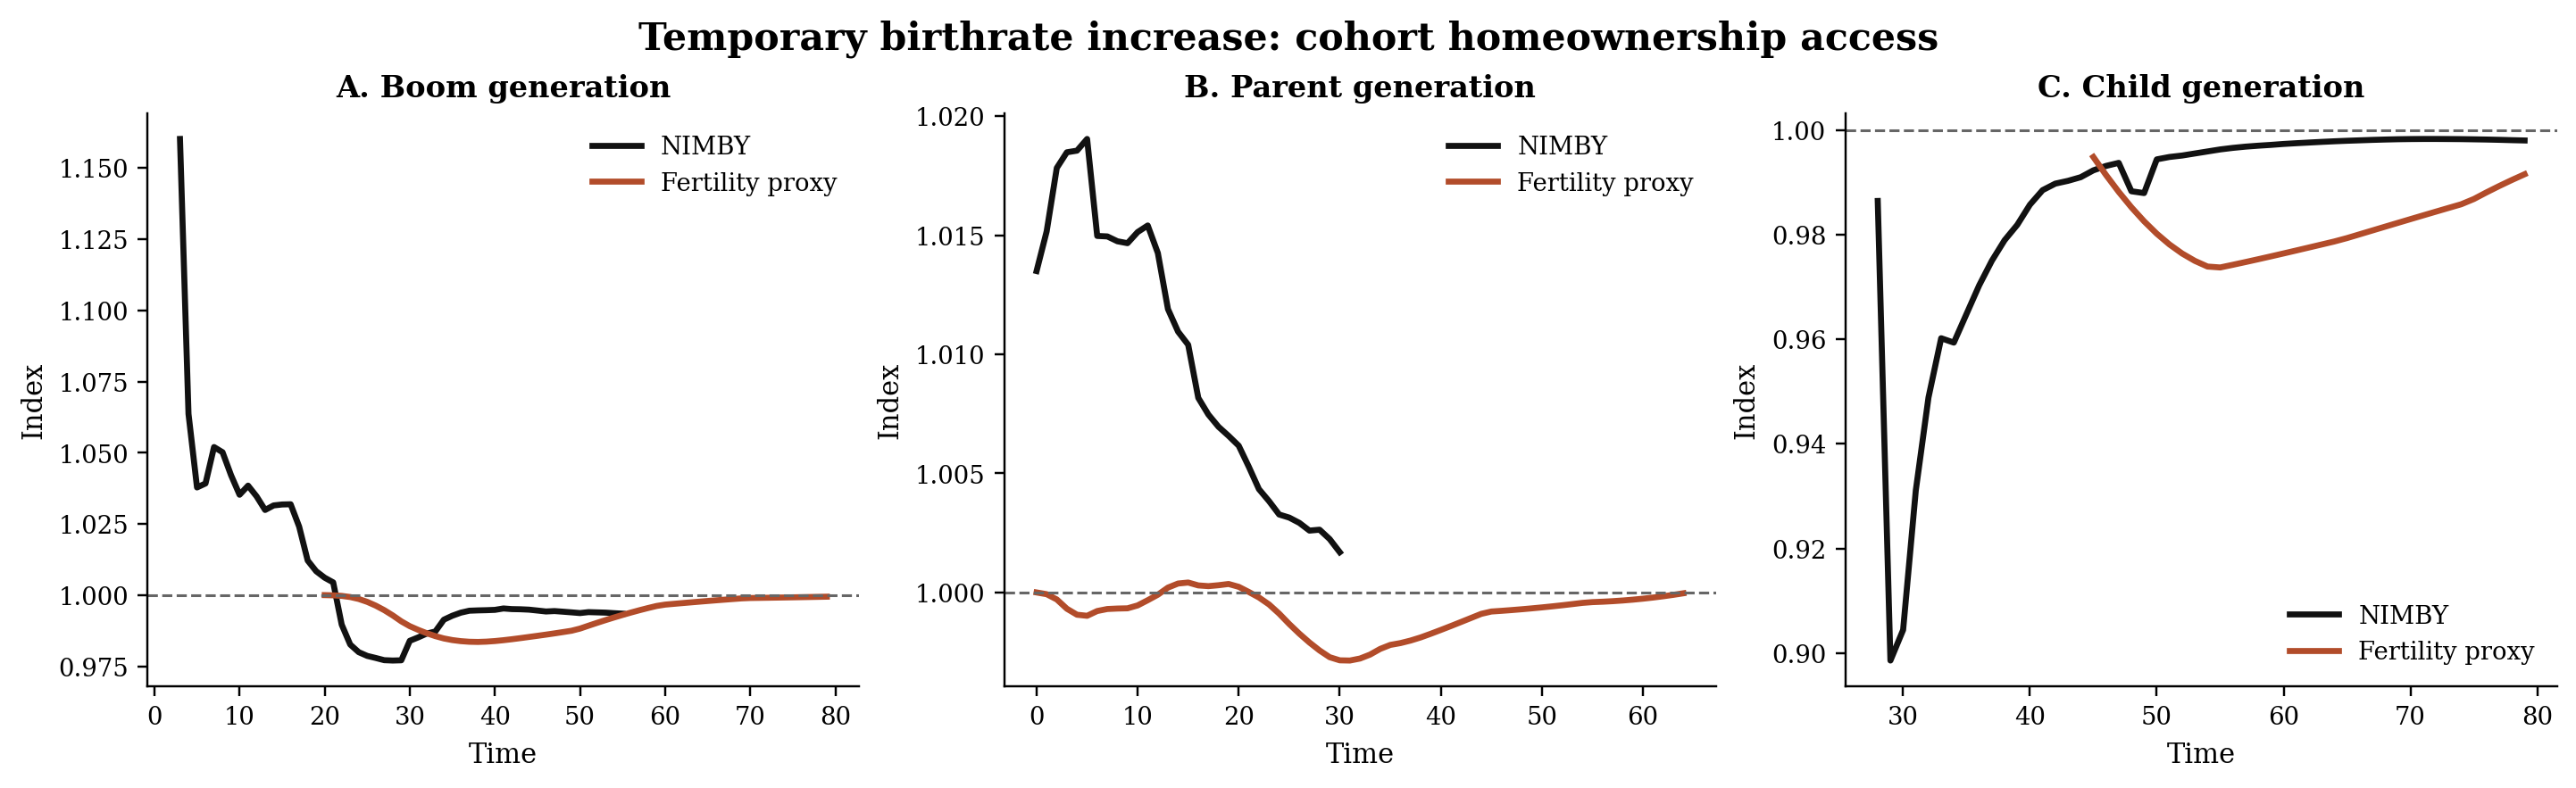
\includegraphics[width=\textwidth]{nimby_vs_fertility_generation_homeownership.png}
\caption{Temporary birthrate increase: cohort homeownership access. The black lines are the
upstream NIMBY cohort homeownership indices. The red lines are fertility-side cohort
homeownership-access proxies built from a common age profile and the model-implied house-price
path. The comparison is informative about lifecycle incidence, but it is not yet a structural
tenure comparison because the project-03 transition block does not solve household tenure choice.}
\end{figure}

\section{Historical fertility validation}

A direct validation question is whether the fertility extension helps the baby-boom experiment
match the subsequent decline in observed fertility. To check that, I use the aggregate historical
weighted-birthrate series from the legacy NIMBY data and compare it to the NIMBY and
fertility-extension transition paths. Figure 5 reports both the raw postwar series and the aligned
post-boom comparison.

The important caveat is that the historical baby boom is more persistent than the toy 10-period
shock used in the model. For that reason, the clean comparison is the shape of the decline after
the boom window rather than exact calendar matching of the peak. Once the historical series is
aligned at 1956 and the model is aligned at period 10, the fertility extension fits the decline
modestly better than the NIMBY line at each horizon considered. Over the first 10, 20, 30, and 40
years of the aligned decline, the RMSE against the historical series is about 0.104, 0.177, 0.218,
and 0.233 in the fertility extension, compared with 0.119, 0.183, 0.226, and 0.243 in the NIMBY
path.

The interpretation is limited but useful. The original NIMBY transition has no mechanism that can
push fertility below baseline after the imposed baby-boom window ends, so it returns immediately to
its baseline level. The fertility extension adds that endogenous post-boom adjustment. The
historical series displays a much larger and longer decline than either model, but the fertility
extension moves the transition in the correct direction.

\begin{figure}[htbp]
\centering
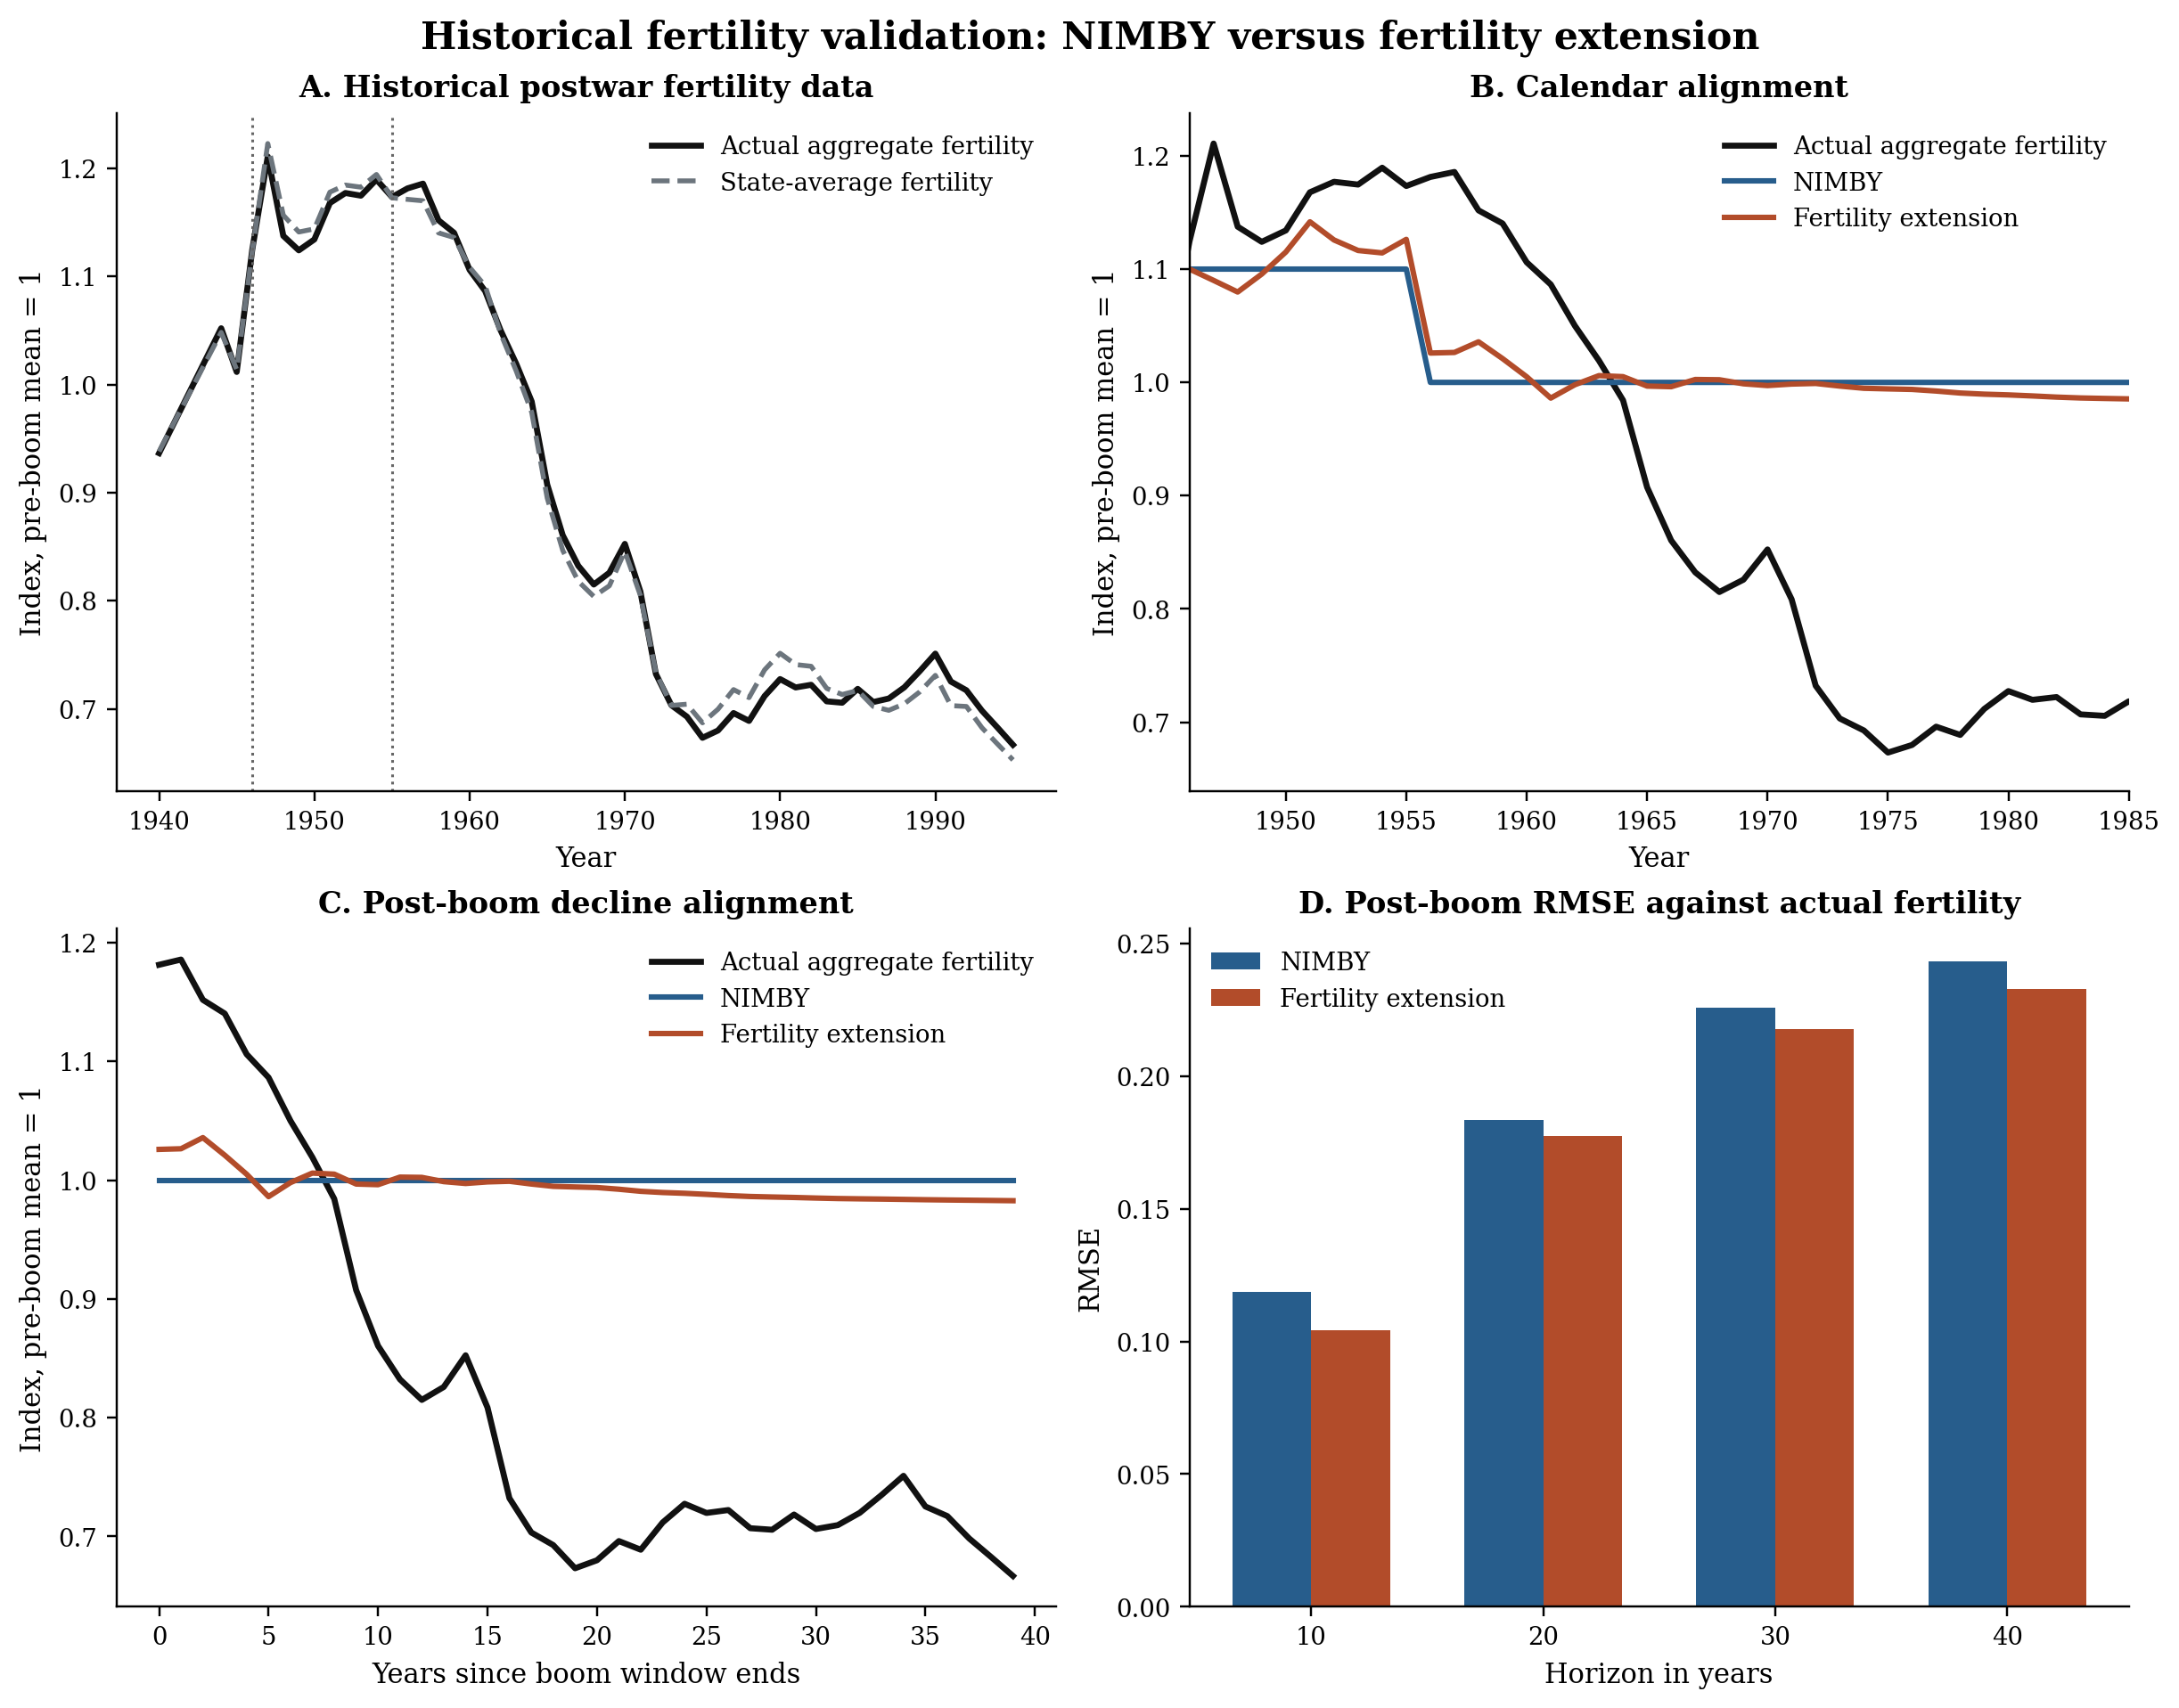
\includegraphics[width=\textwidth]{nimby_vs_fertility_historical_validation.png}
\caption{Historical fertility validation. Panel A plots the aggregate postwar fertility series from
the legacy NIMBY data together with a state-average robustness series. Panel B calendar-aligns the
historical series with the model paths, taking model period 0 as 1946. Panel C aligns the decline
after the boom window, taking 1956 in the data and period 10 in the model as the common starting
point. Panel D reports RMSEs for the aligned post-boom decline.}
\end{figure}

\section{Robustness}

The next question is whether the dynamic comparison is driven by a knife-edge parameter choice
inside the bridge model. Figure 6 reports a bounded robustness sweep around three margins: the
size of the baby-boom shock, the reduced-form price sensitivity of fertility, and the strength of
 family demand in the housing block. The NIMBY side of the sweep uses the project-03 proxy rather
than the upstream IRF because only the benchmark 10 percent shock has been exported from the
original NIMBY transition stack.

The main result is that the central price ranking is robust. Across all three shock sizes, the
fertility extension produces a larger post-boom price response than the NIMBY proxy. At the
benchmark 10 percent shock, the post-boom response is about 0.051 in the fertility extension
against about 0.031 in the NIMBY proxy; at a 30 percent shock the same comparison becomes roughly
0.125 against 0.058. Varying the reduced-form price sensitivity of fertility between 0.10 and
0.30 hardly changes that ranking. Varying the family-demand strength shifts the level of the
fertility price response more noticeably, but again the fertility line remains above the NIMBY
proxy throughout.

The access results are more nuanced than the price results. Stronger shocks make young
homeownership access worse in both models, and by the 30 percent shock the fertility extension has
the more negative young-homeownership trough. But when the change comes from stronger price
sensitivity of fertility or stronger family demand rather than a larger demographic shock, the
fertility extension can partly self-correct through lower later births, so the young-access trough
need not move monotonically with the price response. The robust conclusion is therefore the price
amplification result, not a universal dominance ordering for every access proxy under every
parameter perturbation.

\begin{figure}[htbp]
\centering
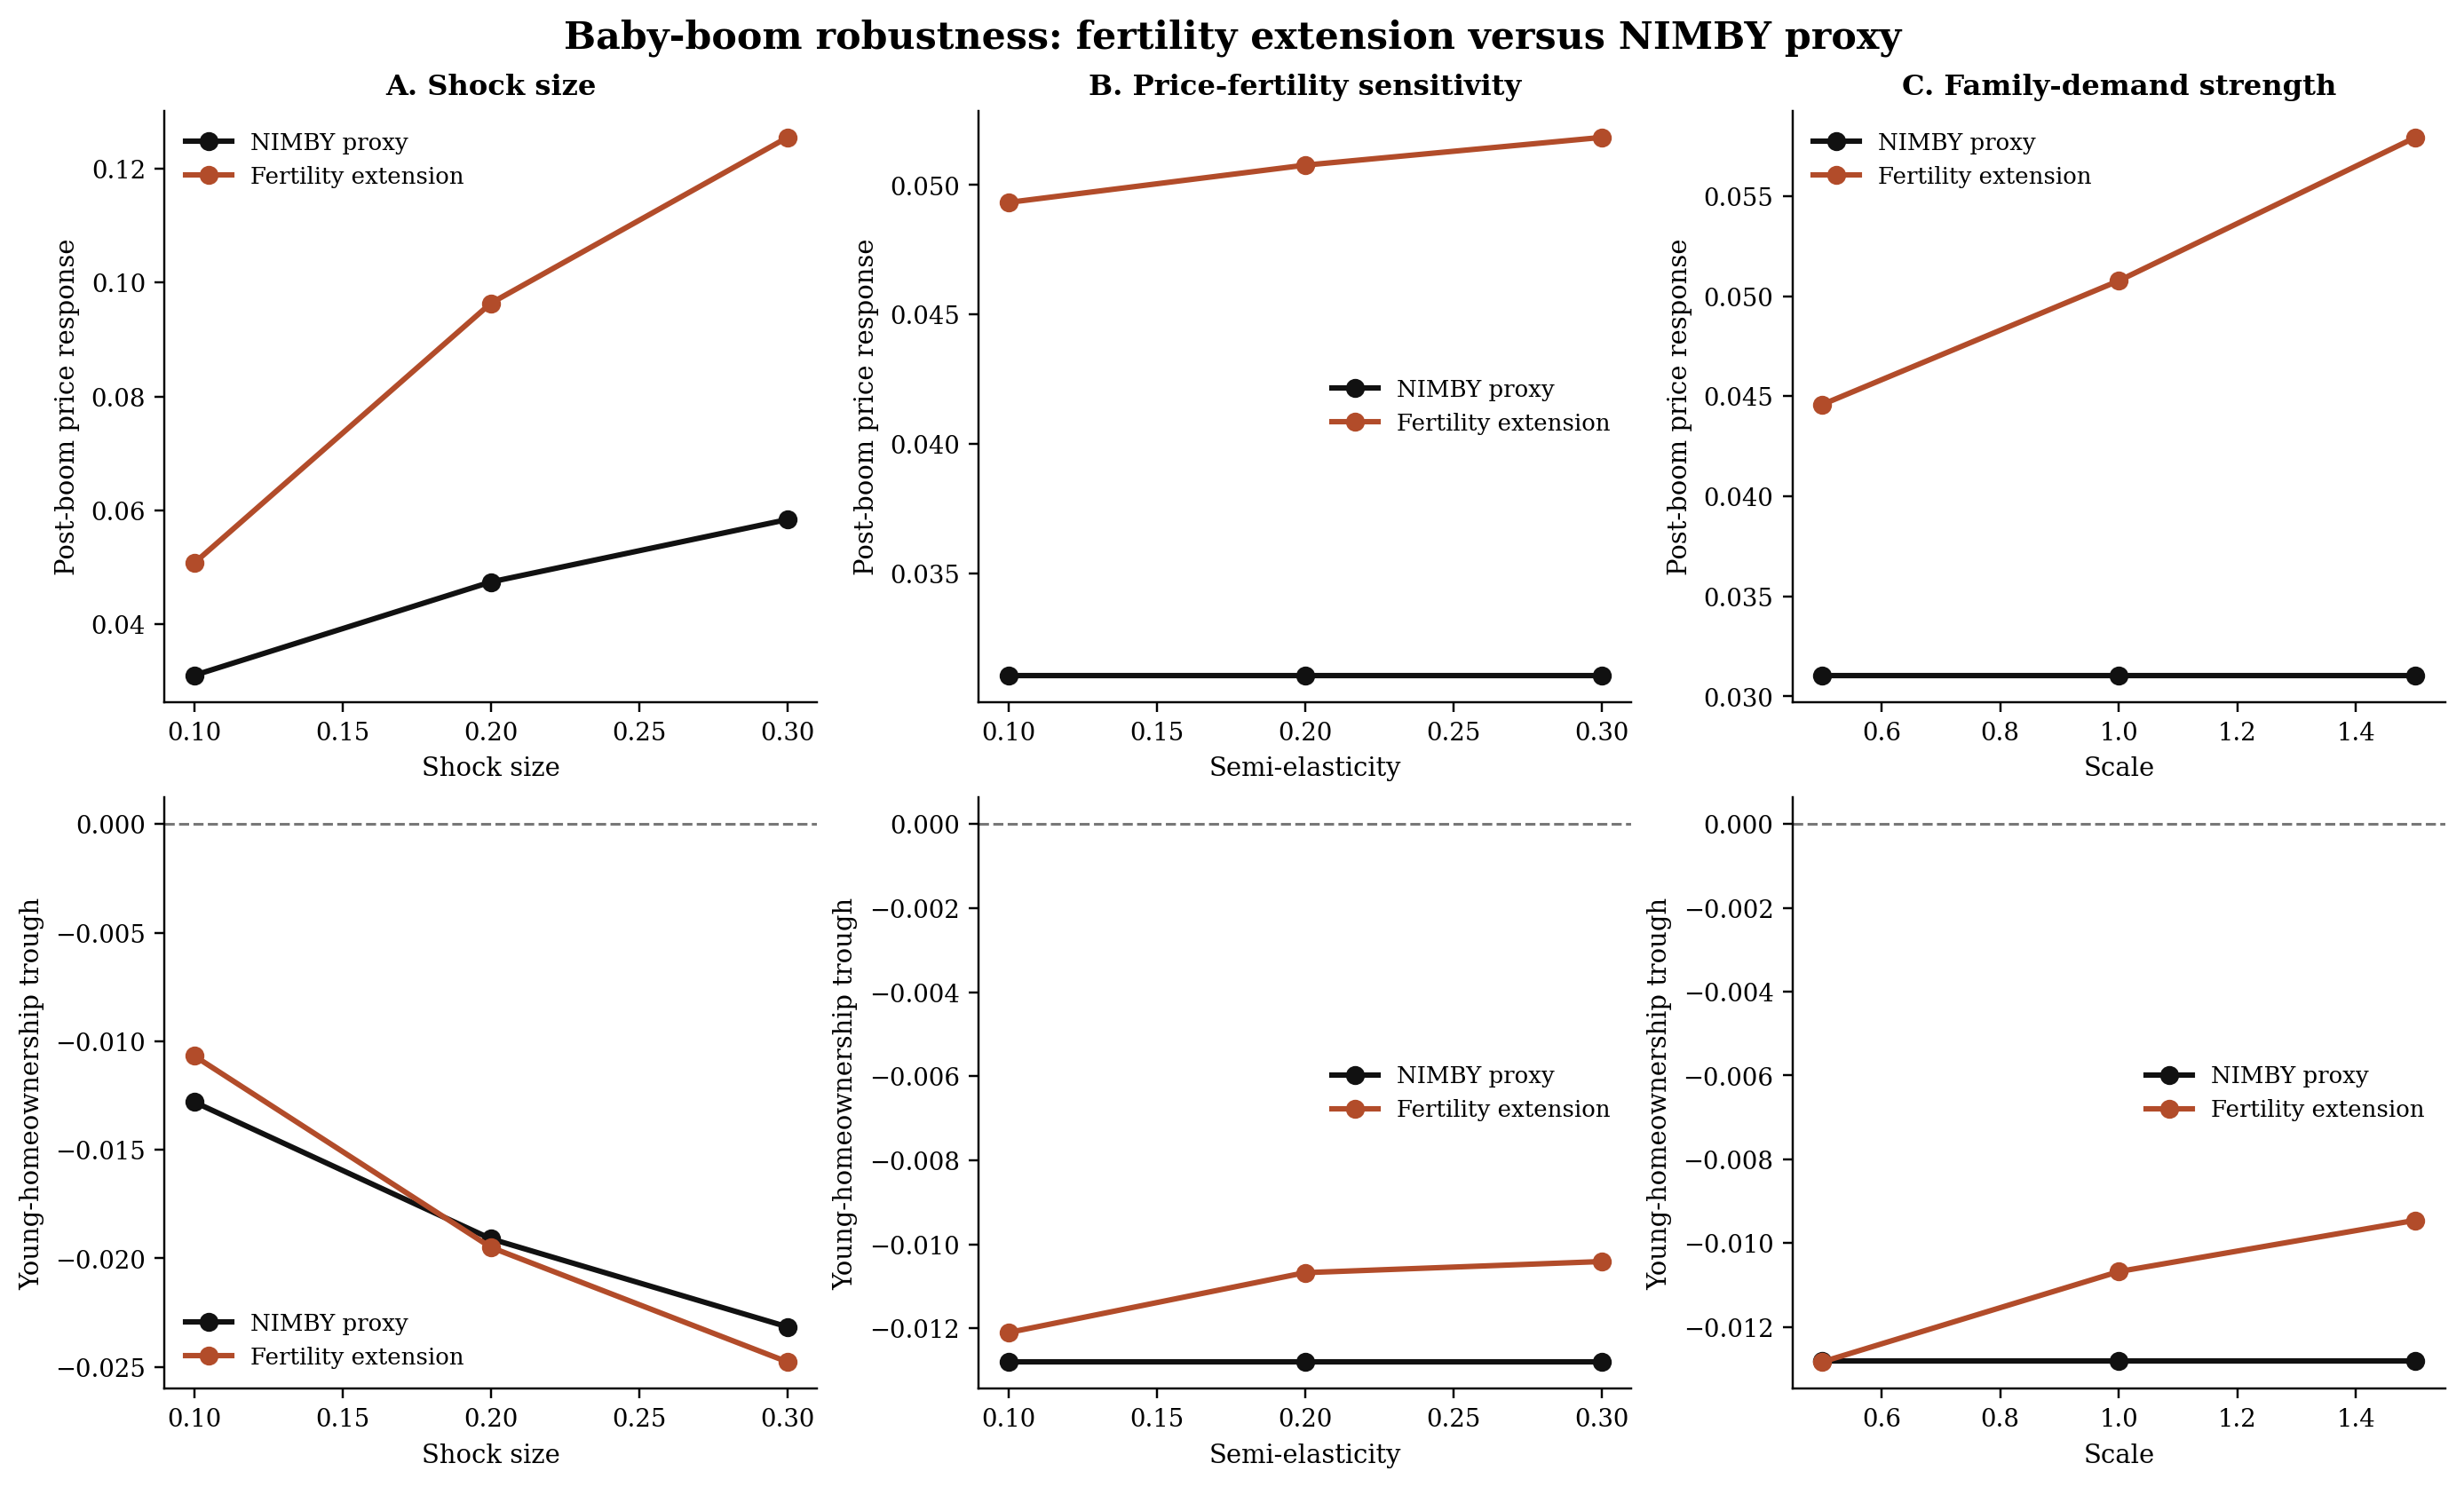
\includegraphics[width=\textwidth]{nimby_vs_fertility_transition_robustness.png}
\caption{Baby-boom robustness. The top row reports the post-boom house-price response under
alternative baby-boom sizes, reduced-form price sensitivities of fertility, and family-demand
strengths. The bottom row reports the corresponding young-homeownership troughs. The black lines
are the project-03 NIMBY proxy; the red lines are the fertility extension.}
\end{figure}

\section{Future demographic projections}

The NIMBY paper also asks what future aging implies for house prices. The accessible upstream
forecast files contain the age-weight scenarios used for that exercise, so Figure 7 feeds those
same projected age weights into the current bridge model. The black lines shut off the
fertility-demand channel and therefore play the role of the NIMBY side of the comparison. The red
lines keep births and children at home in the demand block. This is still a bridge object rather
than the full project-02 forecast solver, but it is the correct next comparison with the files
currently available.

The projected-age results go in the opposite direction from the baby-boom impulse response. Under
all three immigration scenarios, projected aging raises the NIMBY proxy price path but leaves the
fertility path much flatter. In the medium-immigration scenario, the NIMBY proxy reaches a house
price index of about 1.093 by 2050 and about 1.067 by 2100, while the fertility bridge is almost
flat in 2050 at about 1.000 and slightly below its 2020 level by 2100 at about 0.976. The
interpretation is that the family channel pushes in different directions in the short run and the
long run. In the baby-boom experiment, a temporary wave of children at home raises contemporaneous
space demand. In the long projection, aging lowers the mass of family-forming households, so the
fertility channel dampens the aging-driven rise in NIMBY pressure rather than amplifying it.

Panel D of Figure 7 shows that the family-side projection objects remain quantitatively modest in
the medium scenario. Relative to 2020, the fertility-rate index rises by roughly 2 percent in the
2020s, then settles close to one, while the young-homeownership proxy ends slightly above its 2020
level. So the main forecast message is not a future fertility collapse. It is that once the
projected demographic path is dominated by population aging rather than a transitory child wave,
the fertility extension tempers the long-run house-price increase implied by the baseline NIMBY
mechanism.

\begin{figure}[htbp]
\centering
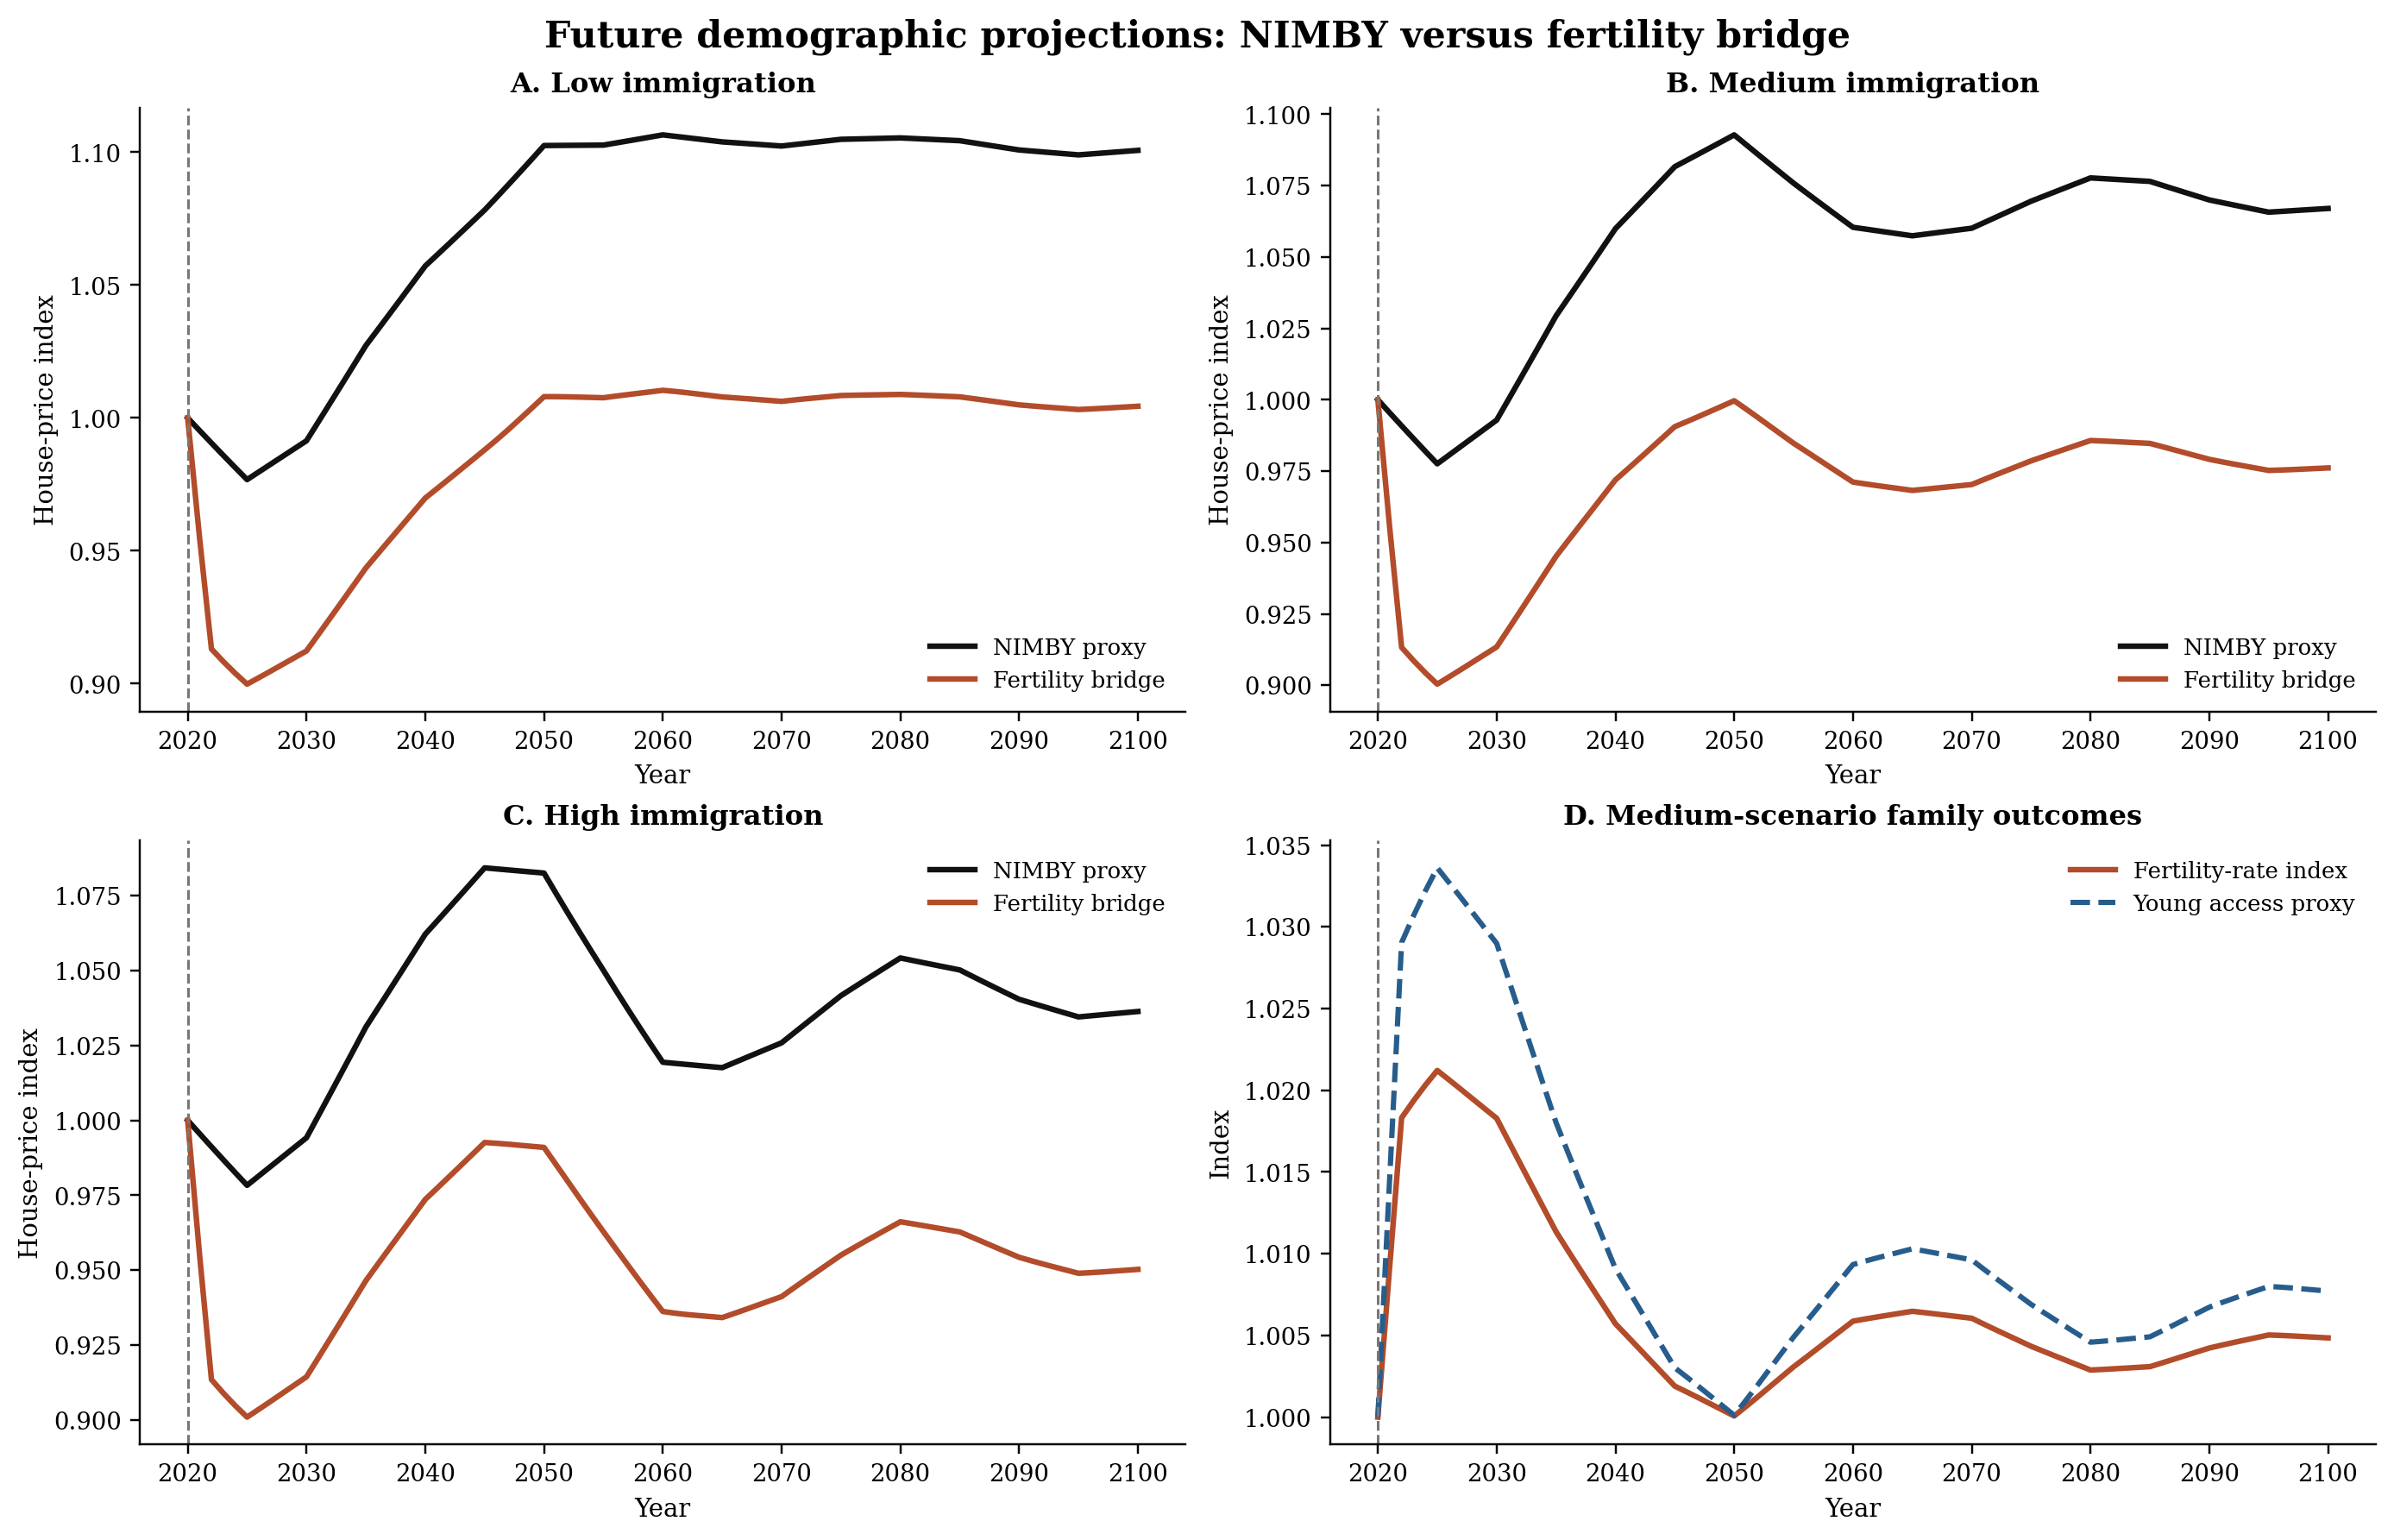
\includegraphics[width=\textwidth]{nimby_vs_fertility_projection_comparison.png}
\caption{Future demographic projections. Panels A--C use the low-, medium-, and high-immigration
age-weight scenarios from the upstream forecast files and compare the NIMBY proxy against the
fertility bridge. Panel D reports the medium-scenario fertility-rate index and young-homeownership
proxy. This is a matched projection bridge rather than the full project-02 forecast solver, but it
uses the same upstream age scenarios on both sides of the comparison.}
\end{figure}

\section{Summary}

The comparison can be summarized in one sentence: the fertility model is not a different voting
model, a different real-estate model, or a different equilibrium concept. It is the NIMBY model
with an augmented household problem in which children at home reduce effective housing services and
births depend on the value of that crowded housing state. Once that family margin is introduced,
the political support schedule shifts toward lower house prices in the steady-state benchmark and
amplifies the medium-run house-price response to a temporary baby boom. That price-amplification
result is robust in the current bridge model. The historical validation exercise shows that the
same fertility margin also moves the post-boom fertility path closer to the long decline in the
aggregate US data, although the fit improvement is modest. The future-projection bridge adds one
final contrast: when the demographic change is long-run aging rather than a temporary child wave,
the fertility channel dampens the rise in projected house prices relative to the NIMBY proxy. The
current transition and forecast blocks still omit the savings and net-worth objects behind the
richer NIMBY cohort-incidence panels, but the basic comparison now covers steady states, baby-boom
transitions, historical validation, bounded robustness, and forward demographic projections.

\appendix

\section{Implementation and verification details}

This note keeps implementation details out of the main text, but three technical points matter for
the benchmark comparison.

First, in the numerical benchmark the birth and no-birth branches are mapped into a smooth birth
probability using
\begin{equation}
\Pr(\text{birth} \mid \mathbf{s}_t) =
\Lambda\left(\frac{V^{F,1}_t(\mathbf{s}_t; q_t)-V^{F,0}_t(\mathbf{s}_t; q_t)}{\varsigma}\right).
\end{equation}

Second, exact nesting is obtained by shutting off the fertility block so that the fertility
extension collapses to the NIMBY benchmark. In the benchmark implementation this means setting
\begin{equation}
\nu_h = \kappa_0 = \kappa_q = \lambda_c = \psi_c = 0
\end{equation}
and removing the active birth branch.

Third, the reported benchmark comparison uses the current steady-state benchmark objects:
\begin{itemize}
\item the fertility benchmark on the household grid $(I,J)=(60,14)$;
\item the upstream NIMBY benchmark on its native grid $(I,J)=(50,10)$;
\item a common price perturbation convention with $rbPos=0.03$.
\end{itemize}

Fourth, the transition comparison uses the upstream NIMBY baby-boom reference from
\begin{verbatim}
C:/Users/Dave_/Dropbox/Zac and David/Code/SteadyState/Mod_IRF/irfs_smoothed.mat
\end{verbatim}
because the smoothed IRF object is not stored in the repo copy. The fertility transition is
generated from the current project-03 transition block under the same temporary 10 percent shock
for 10 periods. House-price responses are reported as deviations from each model's own initial
house-price level so the two transition lines are on a comparable scale.

Fifth, the historical validation uses the legacy aggregate fertility files
\begin{verbatim}
C:/Users/Dave_/Dropbox/Zac and David/Data/merged_birthrates_migrationweights.dta
C:/Users/Dave_/Dropbox/Zac and David/Data/birthrates_updated.dta
\end{verbatim}
and normalizes both historical series by the mean pre-boom birth rate over 1940--1945. The main
comparison is a post-boom shape comparison, not a formal estimation exercise.

Sixth, the robustness sweep is implemented through a Python bridge that reproduces the benchmark
MATLAB policy runs to machine precision before varying the shock size, price sensitivity, and
family-demand strength. The NIMBY side of that sweep is the project-03 proxy rather than a fresh
set of upstream IRFs.

Seventh, the future-demographic projection comparison uses the upstream forecast age weights from
\path{C:/Users/Dave_/Dropbox/Zac and David/Code/SteadyState/Mod_DynamicForecast/loopoutput_forecast.mat}
but the reported comparison is a matched bridge exercise rather than the full project-02 forecast
solver. The black line in Figure 7 is the NIMBY proxy with the fertility-demand channel shut off;
the red line adds births and children-at-home demand under the same projected age path.

Finally, the transition comparison should be read as dynamic mechanism evidence rather than as a
fully unified household-DP transition benchmark. The steady-state comparison is the exact
household-to-household comparison; the transition section shows how the fertility mechanism alters
the original baby-boom experiment under the current project-03 dynamic block. The richer
homeownership objects from the original NIMBY IRFs are now matched by reduced-form
composition-and-affordability proxies on the fertility side, but the transition block still does
not solve a savings problem and therefore does not yet generate directly comparable fertility-side
net-worth panels.

\end{document}
